\section{Evaluation}
\label{sec:eval}
This section evaluates our approach by addressing the following research questions:

\ela{could you please rephrase these questions?! having hard time saying them clearly :-( }
\begin{itemize}
    \item \textbf{RQ1:} How much overhead does computation of set of support add to the proofs? 
    \item \textbf{RQ2:} How dependent is our approach on different tools and proof engines? Does different solvers/ proof engines generate different support set? If so, to what extent are they different?
    \item \textbf{RQ3:} Is there any relationship between the size of a computed support set and 
    solvers/ proof engines? For each model, we have 12 sets of support computed by \texttt{JKind}, and one \emph{minimal} set computed by \texttt{JSupport}; we would like to know which configurations generated sets that are very close or far to the minimal one.
    \item \textbf{RQ4:} How close to minimal are the support sets computed by our algorithm? We would like to know how close 12 sets computed by \texttt{JKind} are to the minimal one.
    \item \textbf{RQ5:} How do different solvers perform on computing support? And, how efficient is it in comparison with \texttt{JSupport}?
\end{itemize} 

\subsection{Analytical Results}
\label{sec:res}
This section answers the aforementioned research questions briefly describing the way the results are analyzed. Note that the results of 10 models with unprovable properties are omitted in calculations. In addition, while analyzing support sets, \texttt{K-induction} settings that timed out were not considered because they failed to prove the properties.

% RQ1: the overhead of support computation on different solvers
\textbf{RQ1.} In general, for timing analyses, from all 13 configurations, we only considered the settings where both \texttt{PDR} and \texttt{K-induction} engines were activated. Since this configuration is a default setting in \texttt{JKind}, we only care about timing while both engines are employed. Therefore, $(4 \times 405) = 1620$ of all 5265 runs have been analyzed to address time-efficiency questions. The overhead is defined as the percentage of the overall runtime is dedicated to support computation:
\mbox{$overhead\_percentage = 100 \times (support\_runtime \div overall\_runtime)$}.
 Table~\ref{tab:overhead} shows the overhead of support computation on different solvers.

\begin{table}
  \centering
  \begin{tabular}{ |c||c|c|c|c| }
    \hline
     solver & min & max & mean & stdev \\[0.5ex]
    \hline
    Z3   & 0.726\% & 45.396\% & 13.414\% & 11.369\% \\[0.5ex]
    Yices &   0.200\%  & 262.254\%   & 47.264\% & 51.193\% \\[0.5ex]
    SMTInterpol& 0.930\% & 268.571\% &  70.500\% & 58.541\%\\[0.5ex]
    MathSAT & 0.502\% & 396.124\% &  71.007\% & 79.990\%\\[0.5ex]
    \hline
  \end{tabular}
  \caption{\small{Overhead of support computation on different solvers}}
  \label{tab:overhead}
\end{table}

\noindent\fbox{%
    \parbox{\textwidth}{%
        In average, computation of support set has less than 50\% overhead. Averagely, if it takes \textit{t} to prove $\mathbb{P}$, it will take \textit{1.5t} to both prove $\mathbb{P}$ and compute its set of support.
    }%
}
 \vspace{9pt}

% RQ2: How dependent is our approach on different tools and proof engines?
\textbf{RQ2.} To answer this question, we analyze the results from different aspects. The following describes methods used for analyzing and their results.

\textbf{(1)} For each model in the benchmarks, the experiments generated 13 different sets of support. We used Jaccard distance to measure dissimilarity between pairwise of these sets:

\begin{center}
$d_J(\small{A}, \small{B}) = 1 - \frac{|A \cap B|}{|A \cup B|} ,\hspace{9pt} 0 \leq d_J(\small{A}, \small{B}) \leq 1$
\end{center}
\vspace{6pt} 

Therefore, we obtained $\binom{13}{2} = 78$ combinations of distances per model. Then, minimum, maximum, average, and standard deviation of the distances were calculated, by which, again, we calculate these four measures among all 405 models. Table~\ref{tab:pairwise-jd} represents the results of this analysis.

\begin{table}
  \centering
  \begin{tabular}{ |c|c|}
    \hline
     min $d_J$ among all models& 0.0 \\[0.5ex]
     \hline
     max $d_J$ among all models& 0.882\\[0.5ex]
     \hline
     mean $d_J$ among all models& 0.027\\[0.5ex]
     \hline
     stdev $d_J$ among all models& 0.062\\[0.5ex]
    \hline
  \end{tabular}
  \caption{\small{Pairwise Jaccard distance between support sets obtained from different configurations}}
  \label{tab:pairwise-jd}
\end{table}

\noindent\fbox{%
    \parbox{\textwidth}{%
        Support sets computed with different solvers and engines have an average Jaccard distance of 0.027, which implies our algorithm has very small dependency on tools and proof algorithms.
    }%
}
 \vspace{9pt}
 
\textbf{(2)} In addition to Jaccard distance, we also measured the similarity among all sets computed in different configurations per model. Let $S_M$ be a set of all support sets computed for model $M$ (i.e. in our experiments, $S_M$ is a set of 13 sets).  We define similarity per model as follows:

\begin{center}
$similarity = \frac{|\bigcap_{i=1}^{13} s_{Mi}|}{|\bigcup_{i=1}^{13} s_{Mi}|}, \hspace{9pt} s_{Mi} \in S_M$
\end{center}
\vspace{6pt} \ela{should see if this formula has any name in mathematics?!}

Needless to say, $0 \leq similarity \leq 1$, and if all the sets in $S_M$ are the same, similarity will be 1. So the more closer to 1 it is, the more similar sets we have. Table~\ref{tab:sim} is a summary of minimum, maximum, average, and standard deviation of similarity among all models. Fig~\ref{fig:sim} also shows similarity in all models.

\begin{table}
  \centering
  \begin{tabular}{ |c|c|}
    \hline
     min of similarity& 0.12 \\[0.5ex]
     \hline
     max of similarity& 1.0\\[0.5ex]
     \hline
     mean of similarity & 0.884\\[0.5ex]
     \hline
     stdev of similarity & 0.165\\[0.5ex]
    \hline
  \end{tabular}
  \caption{\small{Similarity among all models}}
  \label{tab:sim}
\end{table}

\begin{figure}
  \centering
  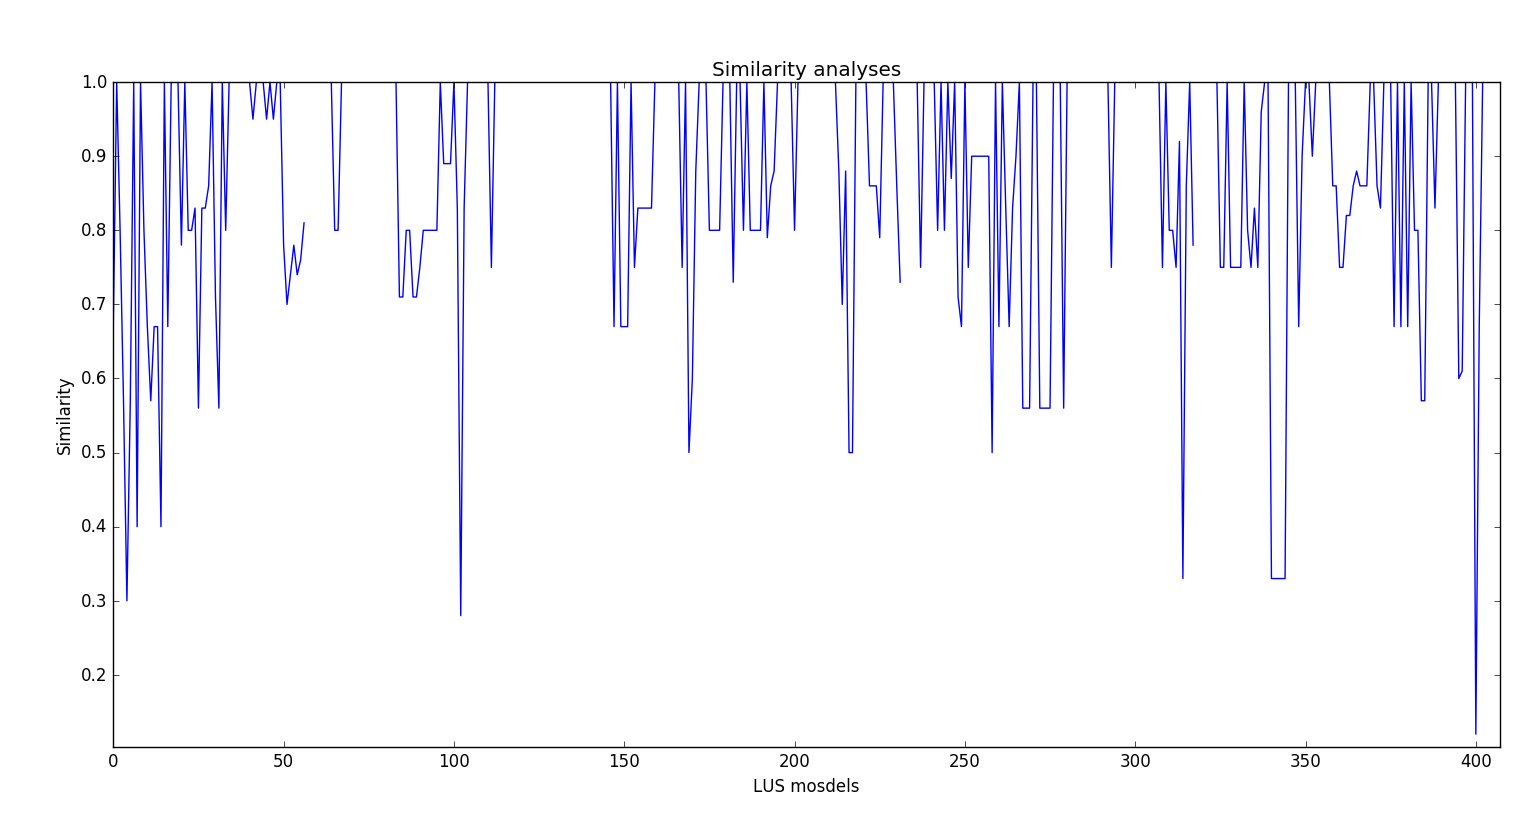
\includegraphics[width=\textwidth]{figs/similarity.png}
  \caption{Similarity measurement for all models}\label{fig:sim}
\end{figure}

\noindent\fbox{%
    \parbox{\textwidth}{%
        An average \textit{similarity} of 0.884 shows that support sets computed in different 
        configurations. So, the dependency of our algorithm to different solvers and proof engines is negligible.
    }%
}
 \vspace{9pt}

\textbf{(3)}
We also calculate a core set of support for each model in the benchmarks; A core set of model $M$ is defined as
$\bigcap_{i=1}^{13} s_{Mi},   hspace{9pt} s_{Mi} \in S_M$, 




% RQ5: overall runtime in JSupport and different solvers
\textbf{RQ5.} In addition to overhead, it is also important to know how efficiently \texttt{JKind} performs on computing set of support in comparison with \texttt{JSupport}. Table~\ref{tab:eff-comp-jsup} compares overall runtime of support computation in different solvers and \texttt{JSupport}.

\begin{table}
  \centering
  \begin{tabular}{ |c||c|c|c|c| }
    \hline
     runtime (sec) & min & max & mean & stdev \\[0.5ex]
    \hline\hline
    JSupport & 2.381 & 165.157 & 21.533 & 23.533 \\[0.5ex]
    Z3   & 0.112 & 42.928 & 2.412 & 5.009 \\[0.5ex]
    Yices &   0.111  & 39.657   & 2.464 & 5.224 \\[0.5ex]
    SMTInterpol& 0.225 & 514.886 &  4.331 & 26.411 \\[0.5ex]
    MathSAT & 0.111 & 43.623 &  2.765 & 5.157 \\[0.5ex]
    \hline
  \end{tabular}
  \caption{\small{\texttt{JKind} runtime with \emph{-support} option in different solvers compared with \texttt{JSupport}}}
  \label{tab:eff-comp-jsup}
\end{table}

%For calculations, we considered all settings where both \texttt{K-induction} and \texttt{PDR} were activated
% then in for all 405 models in everything, we collected runtime info, then calculated min/max/avg/stdev between them
% in other words, there were 4 settings to be considered: z3_both, yices_both, mathsat_both, smtinterpol_both
For 405 models, runtime of support computation in the configurations where both \texttt{K-induction} and \texttt{PDR} were activated has been collected. Fig~\ref{fig:runtimez3} and Fig~\ref{fig:runtimeall} visualize the results.

%\begin{figure}
%\centering
%\begin{tabular}[c]{cc}
%    \begin{subfigure}[b]{0.20\textwidth}
%      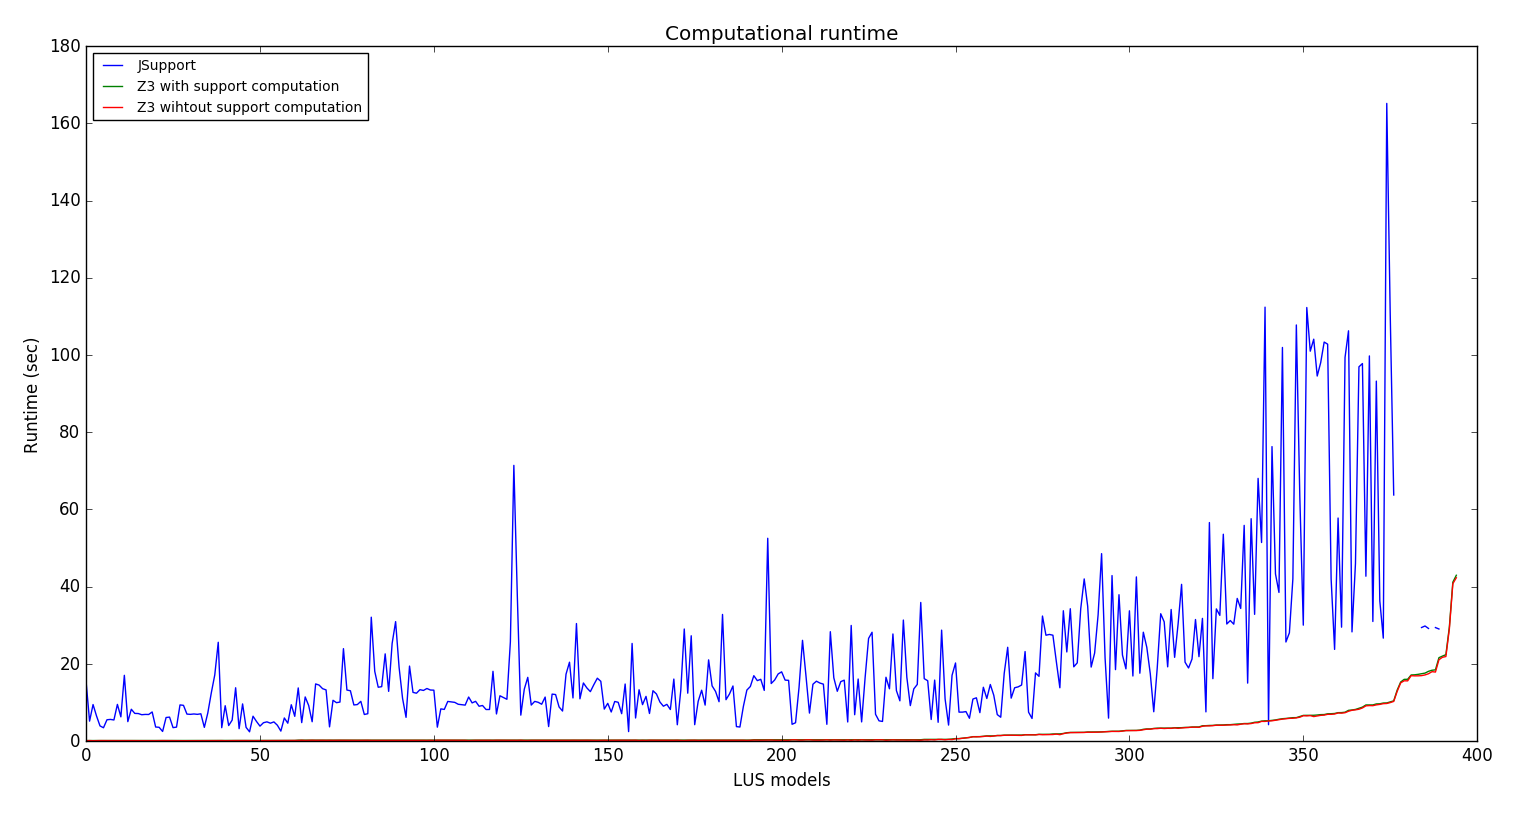
\includegraphics[width=\textwidth]{figs/figure_1.png}
%    \end{subfigure}&
%    \begin{subfigure}[b]{0.20\textwidth}
%      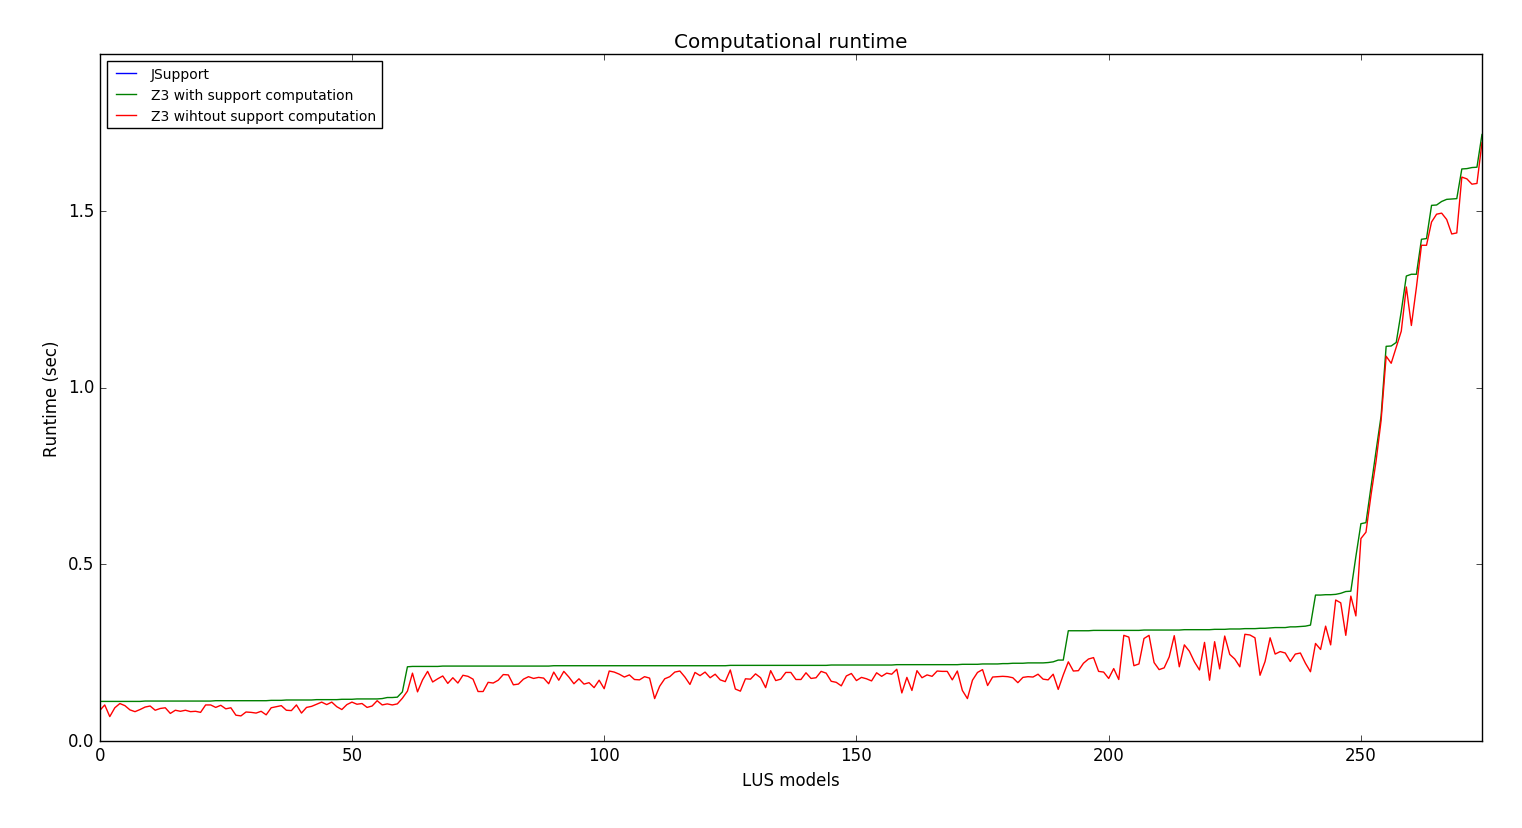
\includegraphics[width=\textwidth]{figs/figure_z3_zoom.png}
%    \end{subfigure}\\
%    \begin{subfigure}[b]{0.20\textwidth}
%      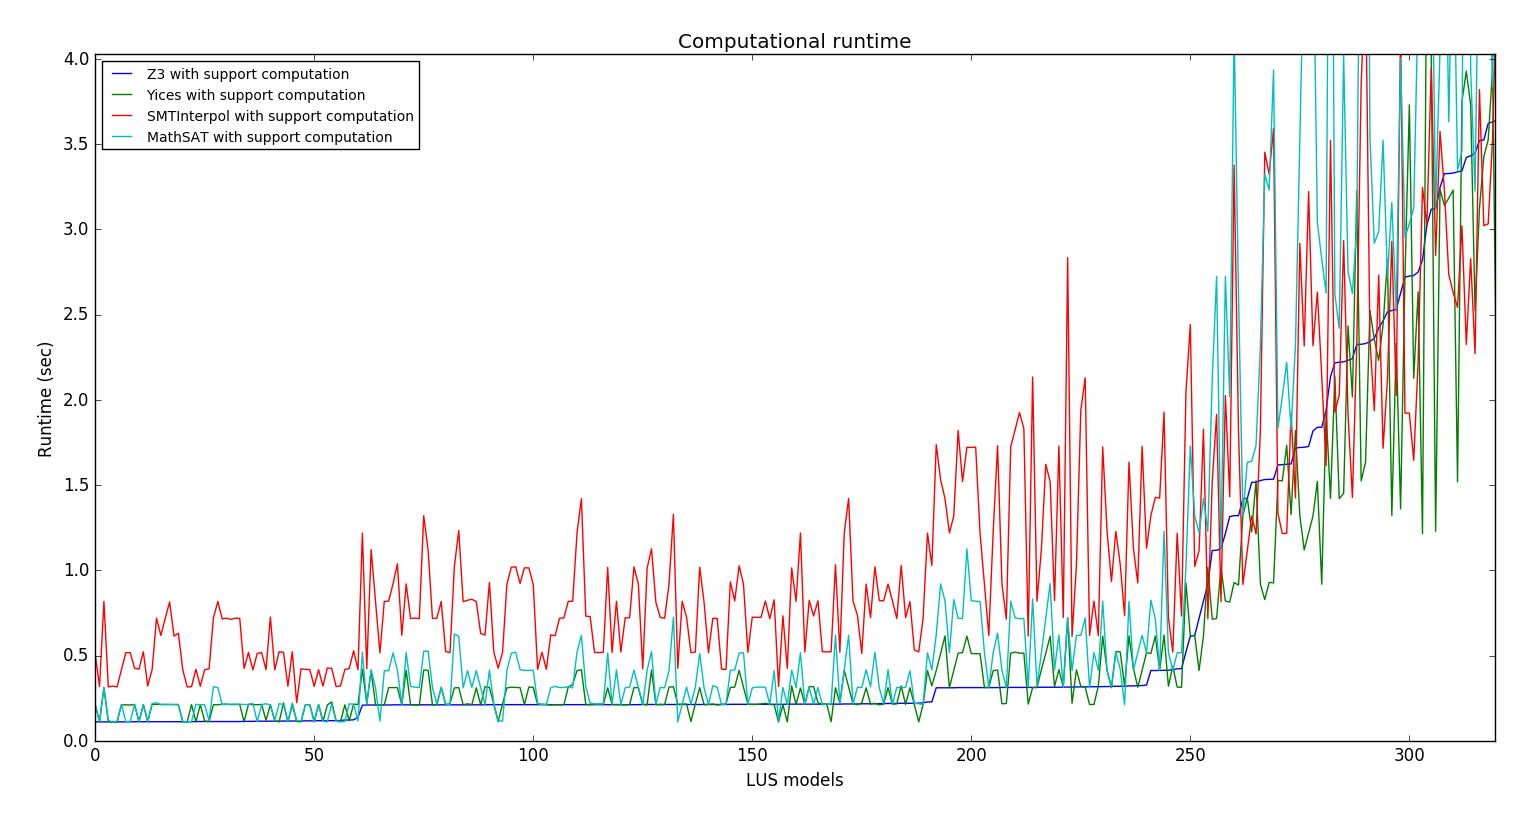
\includegraphics[width=\textwidth]{figs/solvers-support-zoom2.png}
%    \end{subfigure}&
%    \begin{subfigure}[b]{0.20\textwidth}
%      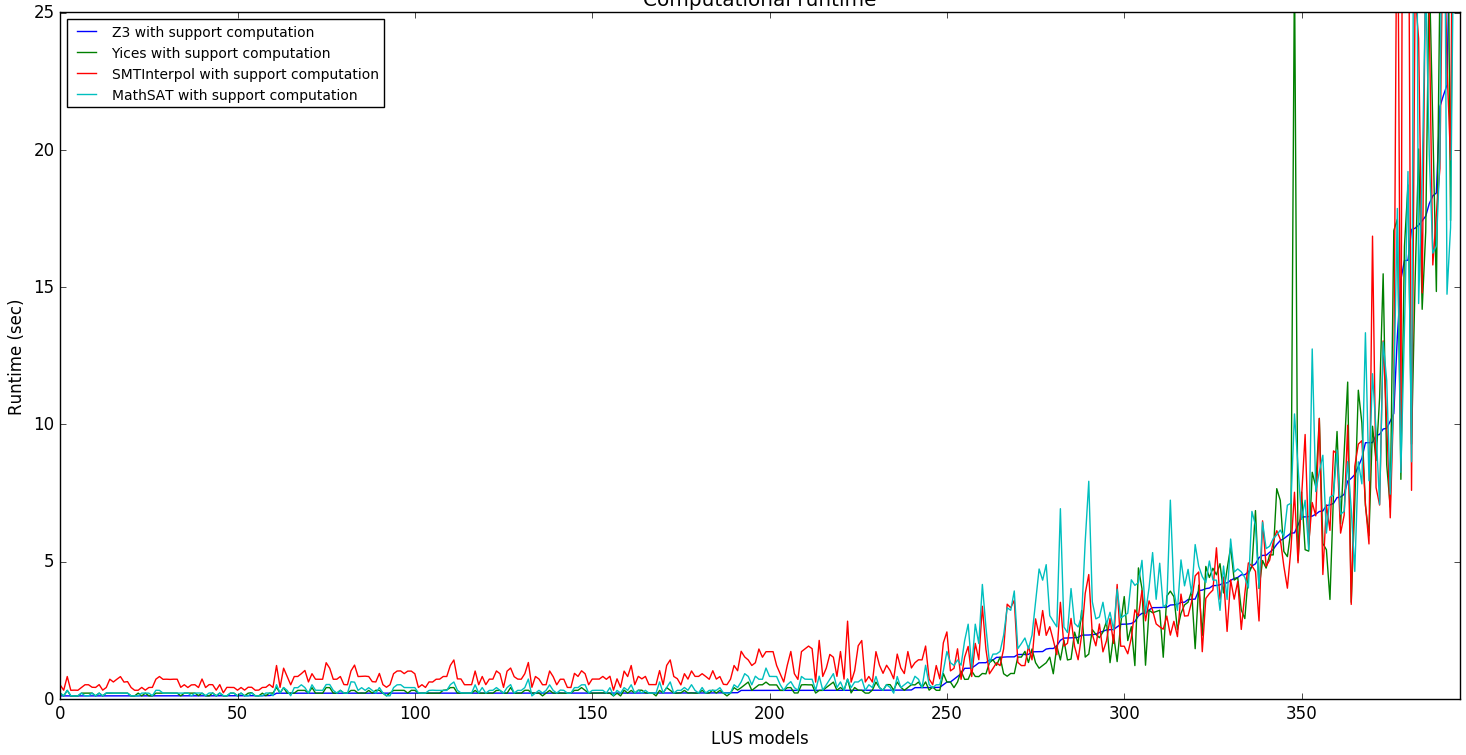
\includegraphics[width=\textwidth]{figs/solvers-support-zoom1.png}
%    \end{subfigure}
%  \end{tabular}
%\caption{\small{Runtime of support computation}}
%\label{fig:runtime}
%\end{figure}
\begin{figure}
  \centering
  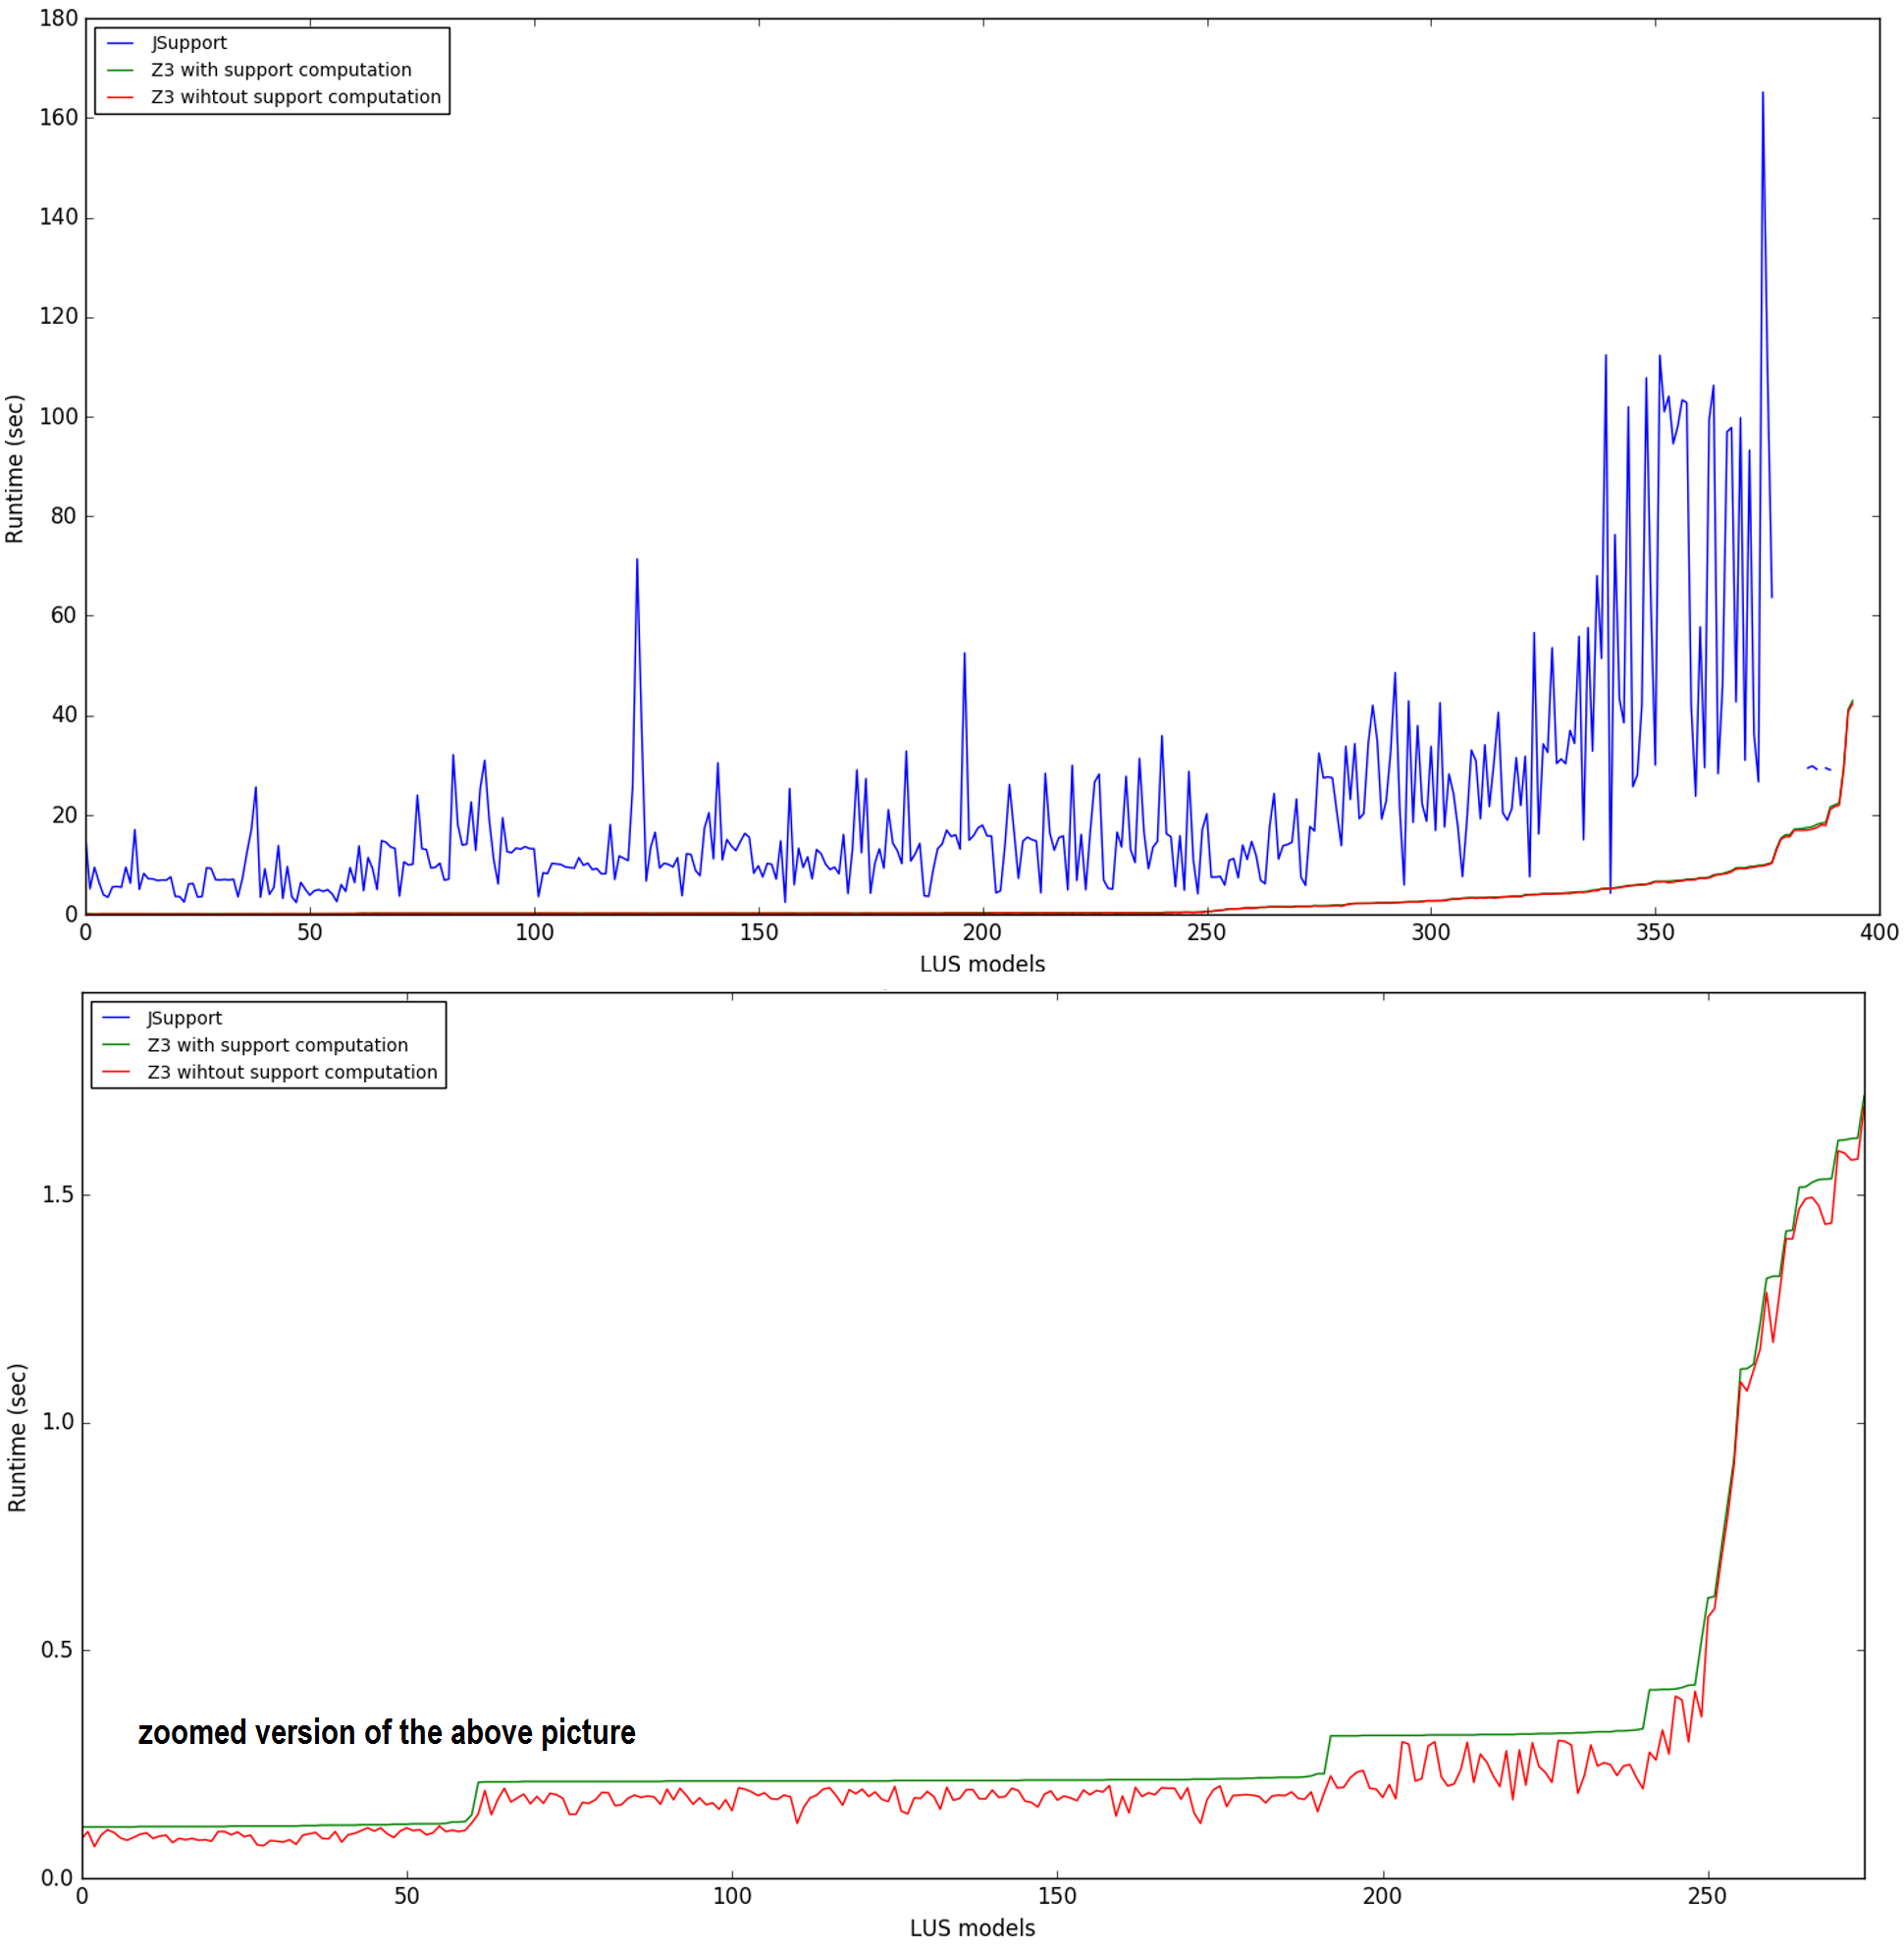
\includegraphics[width=\textwidth]{figs/runtimeZ3.png}
  \caption{\small{Runtime of support computation with \texttt{Z3} and \texttt{JSupport}}}\label{fig:runtimez3}
\end{figure}

\begin{figure}
  \centering
  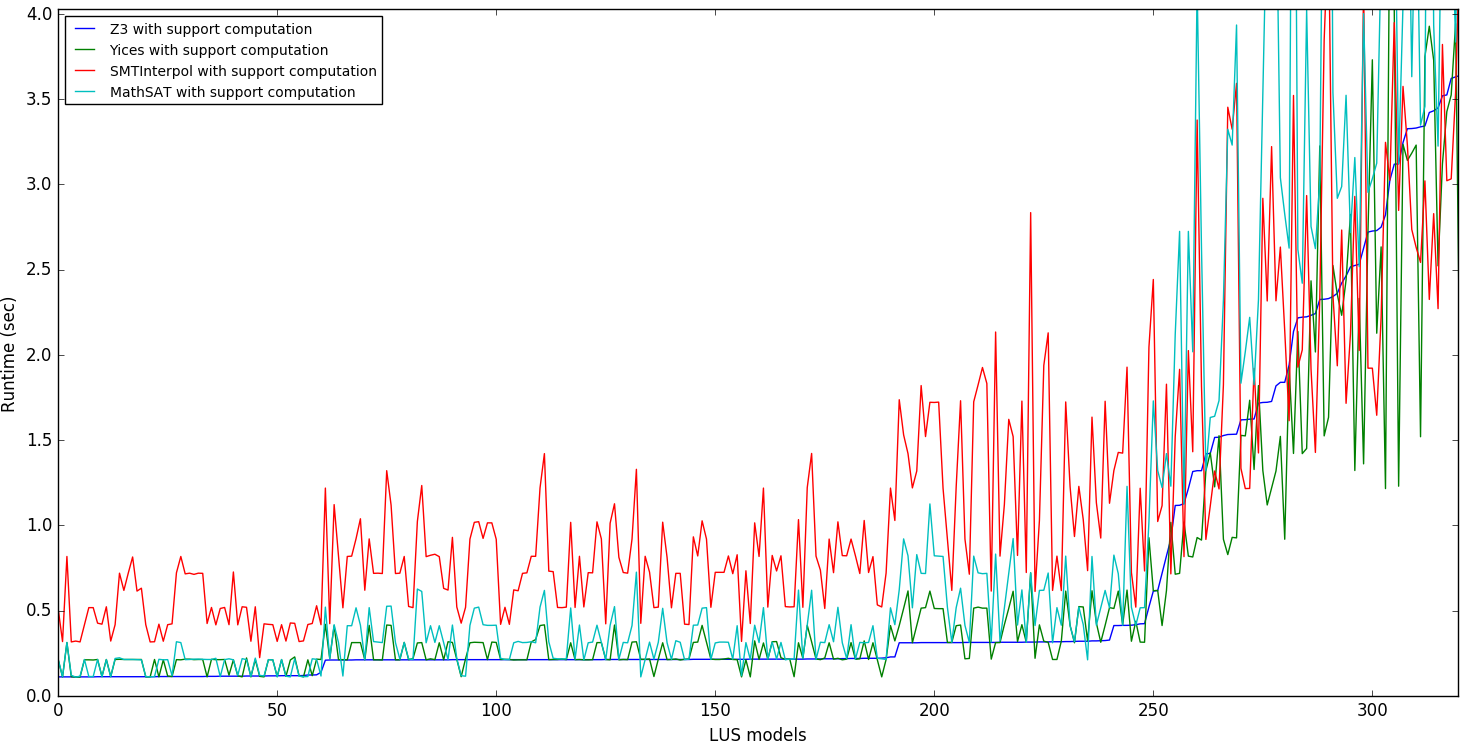
\includegraphics[width=\textwidth]{figs/runtimeAll.png}
  \caption{\small{Runtime of support computation with all solvers}}\label{fig:runtimeall}
\end{figure}
\vspace{6pt}
\noindent\fbox{%
    \parbox{\textwidth}{%
        Time-efficiency of computing support set in \texttt{JKind} is not quite solver-dependent. However, SMTInterpol works less efficiently in comparison with others. 
    }%
}
\noindent\fbox{%
    \parbox{\textwidth}{%
        Support computation by \texttt{JSupport} is much more time-intensive than \texttt{reduce-support} engine.
    }%
}
 \vspace{9pt}